\documentclass[uplatex,dvipdfmx,a4paper,11pt]{jsarticle}

\usepackage{docmute}


% 数式
\usepackage{amsmath,amsthm,amssymb}
\usepackage{bm}
% 画像
\usepackage{graphicx}

\usepackage{multirow}
\usepackage{wrapfig}
\usepackage{ascmac}
\usepackage{xcolor}


\usepackage{makeidx}
\makeindex

\graphicspath{{../../_Figures//}{../../_Figures/Rheology/}}

\usepackage{qrcode}
\setlength\lineskiplimit{0pt}
\setlength\normallineskiplimit{0pt}

\usepackage{qexam}

\usepackage{titlesec}
\titleformat*{\section}{\Large\bfseries}
\titleformat*{\subsection}{\large\bfseries}
\titleformat*{\subsubsection}{\normalsize\bfseries}
\titleformat*{\paragraph}{\normalsize\bfseries}

% ページ設定
% \pagestyle{empty}
% 高さの設定
\setlength{\textheight}{\paperheight}   % ひとまず紙面を本文領域に
\setlength{\topmargin}{-5.4truemm}      % 上の余白を20mm(=1inch-5.4mm)に
\addtolength{\topmargin}{-\headheight}  % 
\addtolength{\topmargin}{-\headsep}     % ヘッダの分だけ本文領域を移動させる
\addtolength{\textheight}{-40truemm}    % 下の余白も20mmに%% 幅の設定
\setlength{\textwidth}{\paperwidth}     % ひとまず紙面を本文領域に
\setlength{\oddsidemargin}{-5.4truemm}  % 左の余白を20mm(=1inch-5.4mm)に
\setlength{\evensidemargin}{-5.4truemm} % 
\addtolength{\textwidth}{-40truemm}     % 右の余白も20mmに
% 図と本文との間
%\abovecaptionskip=-5pt
%\belowcaptionskip=-5pt
%
% 全体の行間調整
% \renewcommand{\baselinestretch}{1.0} 
% 図と表
%\renewcommand{\figurename}{Fig.}
%\renewcommand{\tablename}{Tab.}
%

% \makeatletter 
% \def\section{\@startsection {section}{1}{\z@}{1.5 ex plus 2ex minus -.2ex}{0.5 ex plus .2ex}{\large\bf}}
% \def\subsection{\@startsection{subsection}{2}{\z@}{0.2\Cvs \@plus.5\Cdp \@minus.2\Cdp}{0.1\Cvs \@plus.3\Cdp}{\reset@font\normalsize\bfseries}}
% \makeatother 

\usepackage[dvipdfmx,%
 bookmarks=true,%
 bookmarksnumbered=true,%
 colorlinks=false,%
 setpagesize=false,%
 pdftitle={数式に頼らない直感的理解による材料設計のためのレオロジー⼊⾨},%
 pdfauthor={佐々木裕},%
 pdfsubject={},%
 pdfkeywords={レオロジー; 材料設計; }]{hyperref}
\usepackage{pxjahyper}

\usepackage{plext}

\usepackage{niceframe} 
\usepackage{framed}
\newenvironment{longartdeco}{%
  \def\FrameCommand{\fboxsep=\FrameSep \artdecoframe}%
  \MakeFramed {\FrameRestore}}%
 {\endMakeFramed}
 
\usepackage{siunitx}

\newcommand{\rmd}{\mathrm{d}}

\usepackage[inline]{showlabels}

\begin{document}

\section*{この章の内容}

この章では、「レオロジーをはじめる前に」として、レオロジーを理解するために必要となる準備を行っていきます。
具体的には、数学及び物理の基本となるような考え方についての確認から手を付けていきます。

以下に、この章で議論する内容について簡単にまとめました。

	\begin{boxnote}
		\large
		\begin{itemize}
			\item 数学的な事項の確認
			\begin{itemize}
				\item 数学的に書き表すときに基本となる「関数」について
				\item 事象を単純化して考えるときに重要な「線型性」
			\end{itemize}
			\item 物理的に考えるときに必要になること
			\begin{itemize}
				\item 物理モデルと線型性
				\item 物理モデルを理解するために、「量」、「次元」、「単位」
			\end{itemize}
		\end{itemize}
	\end{boxnote}

\section{数学的な事項の確認から}

具体的なレオロジーの議論に入る前に、これからの議論に必要となる数学の基礎的な事項について確認していきましょう。
ここでは、それほど難しいものを考えているわけではありません。
レオロジーを理解するために、どうしても必要となる中学から高校レベルの基本的なことを思い出していただくことになります。

具体的には、「関数と線型\index{せんけい@線型}性」ということについて少しずつイメージを明確にしていくようにしましょう。

\subsection{関数\index{かんすう@関数}について}
\subsubsection{直感的理解}
まず、関数を直感的に理解することから始めます。
\begin{figure}[htb]
	\begin{center}
		\begin{minipage}{0.5\textwidth}
			\large
			\begin{itembox}[l]{関数とは?}
				\begin{itemize}
					\item ある変数 $x$ に依存して決まる出力 $y$ を決める方法(右上)
					\item 入力 $x$ に対して出力 $y$ を与える変換装置(ブラックボックス)のようなもの(右下)
				\end{itemize}
			\end{itembox}
			
		\end{minipage}
		\begin{minipage}{0.4\textwidth}
			\begin{center}
			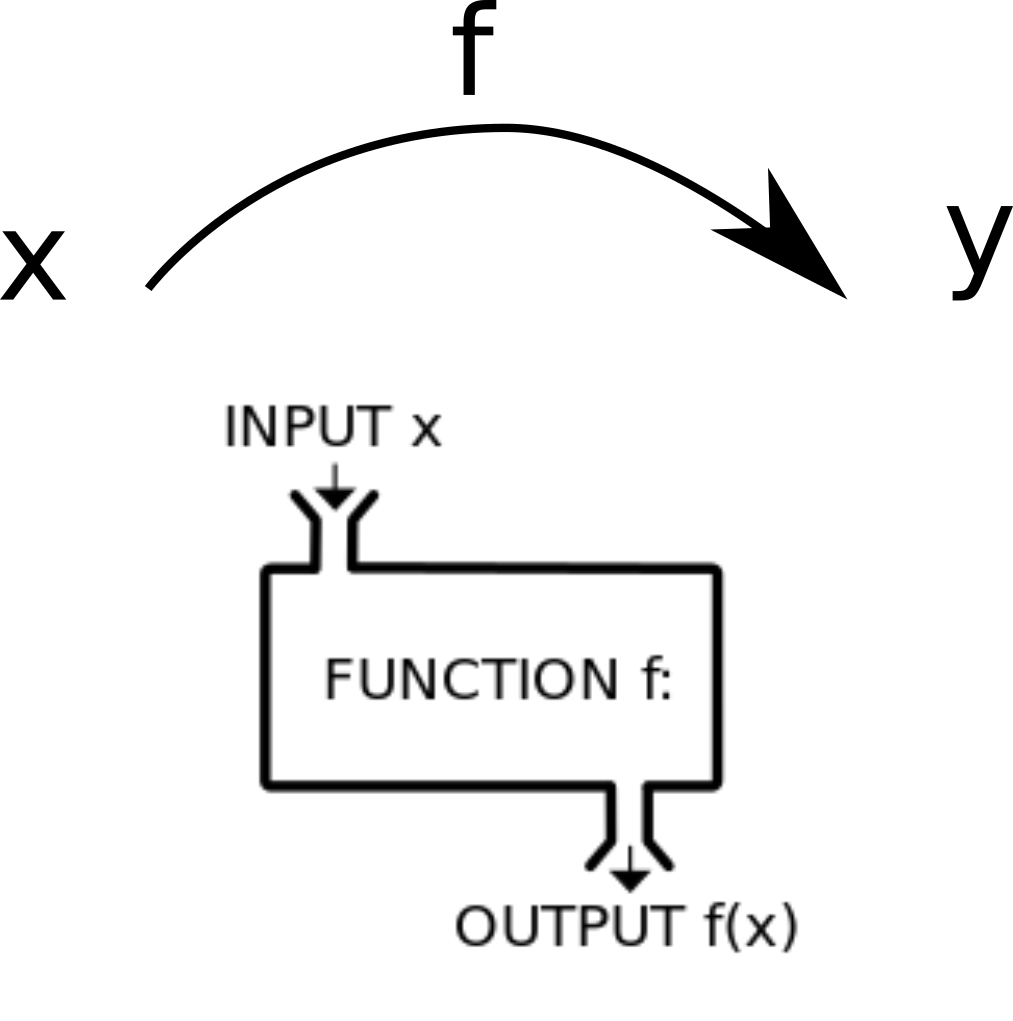
\includegraphics[width=.9\textwidth]{function.png}
			\end{center}
		\end{minipage}
		\caption{関数とは}
		\label{function}
	\end{center}
\end{figure}

関数とは、2つの変数 $x$ と $y$ があり、入力を $x$ で表したときに、その出力 $y$ を決定する規則というようなイメージと捉えることができます。
一般に、関数は、英語の function の頭文字を使って $f$ で表され、どの変数を入力として用いている関数であるかをカッコの中に変数を書くことにより示します。
\begin{align*}
	y&=f(x) \\
	\text{出力}&=\text{関数} \left(\text{入力} \right)
\end{align*}

関数の役割を考えてみると、入力を変換装置に入れた結果として出力が現れるわけですから、入力と出力との間の関係を表していると考えることもできます。

\subsubsection{関数と写像}
また、関数\index{かんすう@関数}というのは、数の集合に値を取る写像の一種と考えることもできます。

定義域と呼ばれる左の集合から、値域となる右の集合への射影を行う方法が、関数ということになります。
\begin{figure}[htb]
	\begin{center}
		\begin{minipage}{0.45\textwidth}
			\large
			\begin{itembox}[l]{集合と関数}
				\begin{itemize}
					\item 左の集合(定義域)から
					\item 右の集合(値域)へ
					\item 射影する方法が関数
				\end{itemize}
			\end{itembox}
		\end{minipage}
		\begin{minipage}{0.45\textwidth}
			\begin{center}
			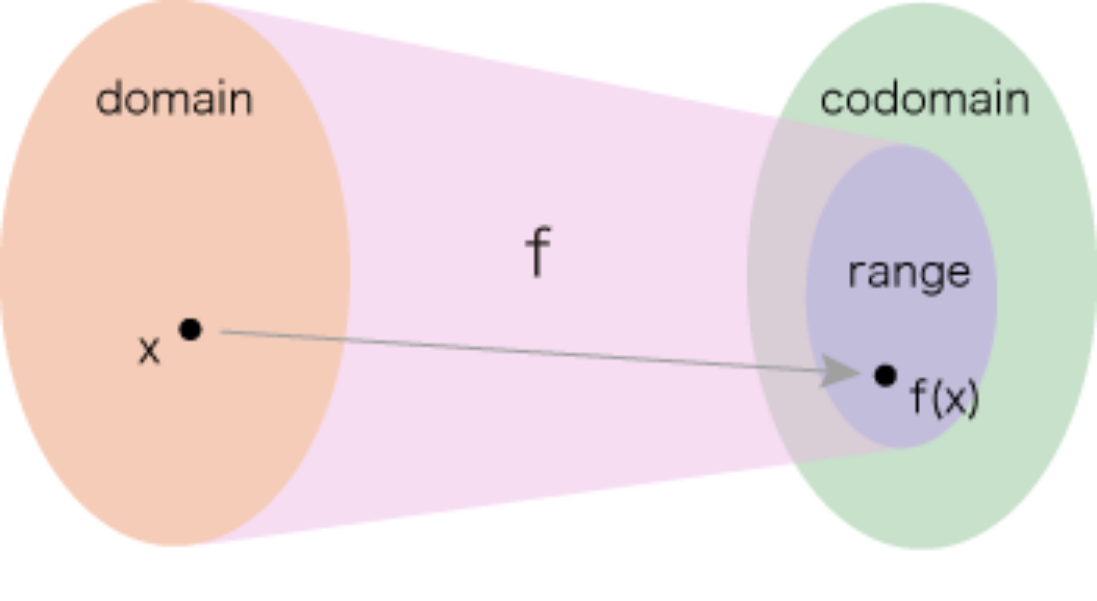
\includegraphics[width=.9\textwidth]{function_2.png}
			\end{center}
		\end{minipage}
		\caption{関数と写像}
		\label{function_2}
	\end{center}
\end{figure}

\subsubsection{グラフとは}
グラフ\index{ぐらふ@グラフ}とは、入力と出力との関係を平面図
\footnote{
	本当は、二次元とは限らずに多次元空間で表したグラフも使われていますが、直感的な理解は平面図にまさるものはありません。
}に示したものであり、視覚的にその関係を理解しやすくしたものと考えることができます。

具体的には、入力 $x$ に対応して決まる出力の点を平面上にたくさん書き込んで、それを連続的に(直線または曲線で)つないだものがグラフとなります。
\begin{figure}[htb]
	\begin{center}
		\begin{minipage}{0.45\textwidth}
			\large
			\begin{itembox}[l]{関数を表すグラフ}
				\begin{itemize}
					\item 横軸が入力
					\item 縦軸が出力
					\item 関数の値を連続的に
				\end{itemize}
			\end{itembox}
		\end{minipage}
		\begin{minipage}{0.45\textwidth}
			\begin{center}
			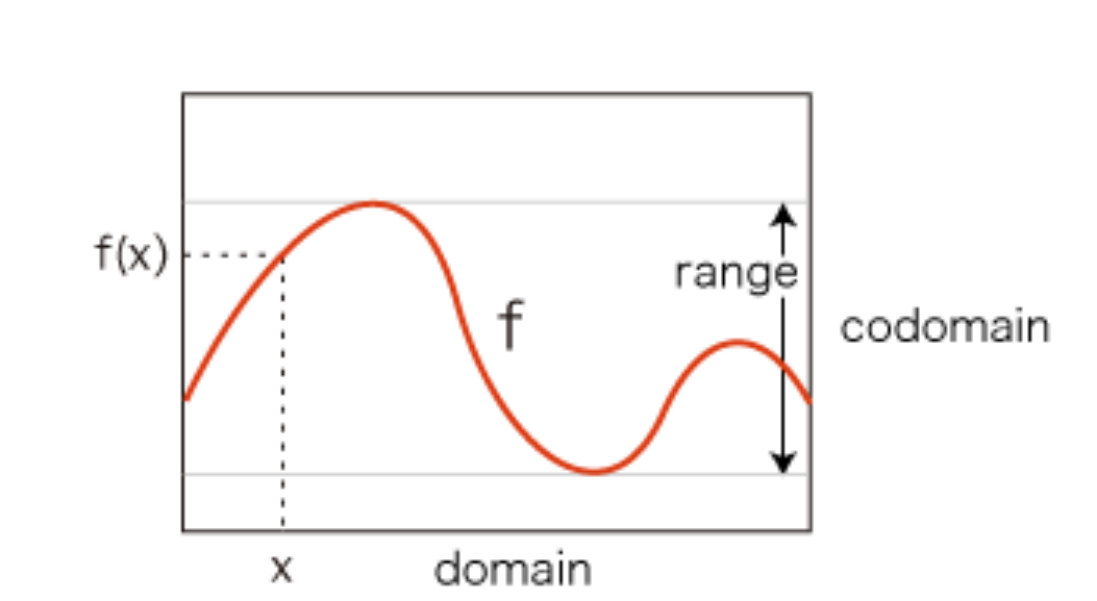
\includegraphics[width=\textwidth]{function_3.png}
			\end{center}
		\end{minipage}
		\caption{関数とグラフ}
		\label{function_3}
	\end{center}
\end{figure}


図 \ref{function_2} の右に示した集合間の写像を二次元のグラフに表すと、図 \ref{function_3} のように値を決める赤い曲線が関数を表すというイメージとなります。
このグラフに表した関数の形を見ることで、入力と出力との関係を直感的に理解することができます。

\subsection{線型\index{せんけい@線型}という意味を理解しよう}

\subsubsection{線型とは?}
線型\index{せんけい@線型}という言葉を直感的にイメージすると、グラフに表した時に原点を通る直線となるような性質と捉えることができます。

数学的にもう少しだけきちんというと、関数などの演算(写像)$f$ が以下に示した2つの性質を満たすときに、$f$ のそのような性質を線型性と呼ぶことになります。
\large
\begin{itembox}[l]{線型を表す性質}
	\begin{itemize}
		\item 加法性:任意の $x,y$ に対して、
		\begin{align*}
			f(x+y)=f(x)+f(y)
		\end{align*}
		\item 斉次性:任意の $x,a$ に対して、
		\begin{align*}
			f(ax)=af(x)
		\end{align*}
	\end{itemize}
\end{itembox}
\normalsize

線型\index{せんけい@線型}性を示す関数はたくさんありますが、以下のように表される一次方程式が代表的なものとなります
\footnote{
	定数項が入った $y=ax+b$ は同様に直線関係を表しますが、このままでは斉次性が成り立たないことに注意してください。

	なお、$y'=y-b$ と変数変換すれば、$y'=ax$ となり線型となります。
}。
\begin{align*}
	y=ax
\end{align*}

これは、入力の大きさが二倍になれば、出力も二倍になるという比例の関係を表しています
\footnote{
	比例の関係を式に表すという授業は、今は小学校5年生で習っているようです。
}。
また、加法性を利用して、小学校の応用問題としての旅人算
\footnote{
	例えば、「A君とB君が 3km 離れた地点から向かい合って同時に出発しました。A君は毎分 30m、B君は毎分 70m で歩いたとすると、二人が出会うのは出発してから何分後ですか。」というような問題です。
}にも使われます。

\subsubsection{線型\index{せんけい@線型}性の意味}

では、線型\index{せんけい@線型}性が成立することで何が嬉しいのでしょうか。

小学校レベルの簡単な問題を考えてみましょう。
「水道の栓を開けて、浴槽に水を溜めています。5 分間流して、100L の水が溜まりました。」
このとき、「1 分間流したときには、何 L 溜まっていたでしょう?」と聞かれたとすると、比例の関係から $1 \text{分} \times 100 L /5 \text{分}= 20 L$ と答えることができ、これは、\textbf{過去を推定}していることになります。
同様に、「10 分では、何 L 溜まるでしょう?」では、\textbf{未来のことを予測}することができます
\footnote{
	これは、暗黙のうちに斉次性を利用していることになります。
}。

また、「浴槽に二つの蛇口から水を溜めていきます。A という蛇口からは 1 分間で 20 L、B という蛇口からは 5 分間で 150 L の水を貯めることができます。両方の蛇口から同時に水を溜めたとき、10 分間では何 L の水が溜まるでしょう?」というような問題でも、加法性と斉次性を利用すれば簡単に解くことができます。

すなわち、線型\index{せんけい@線型}性が成立する(と仮定する)ことで、\textbf{事象を重ね合わせながら過去や未来の値を決める}ことが容易にできるわけです。
\large
	\begin{itembox}[l]{線型性の意味}
		\begin{itemize}
			\item 比例の関係を利用して、
			\begin{itemize}
				\item 過去を推定。
				\item 未来を予測。
			\end{itemize}
			\item 加法性と斉次性を利用して、
			\begin{itemize}
				\item 事象を重ね合わせて、推定や予測。
			\end{itemize}
		\end{itemize}
	\end{itembox}
\normalsize

\section{物理的に考えるときに必要になること}

\subsection{物理モデル\index{ぶつりもでる@物理モデル}と線型\index{せんけい@線型}性}
続いて、物理モデルという言葉について考えてみましょう。

ここまで、モデルという言葉を特別に定義することなく使ってきましたが、本来は、型や模型という意味を持っていて、
それが転じて、手本や模範という意味でよく使われる言葉です。
また、「事象や理論の成り立ちを説明するための簡単で理解しやすい概念」と解説されることもよくあります。
例えば、「地動説」を説明するために、太陽の周りを惑星が回るという「太陽系モデル」が提案され、
経済活動においても利益を最大化するためにいろいろな「ビジネスモデル」が考案されるわけです。
また、「モデルとは、対象とする事象を簡略化して、その本質を表したもの」という表現をされることもあります。

\subsubsection{物理モデル\index{ぶつりもでる@物理モデル}とは}
そして、対象を物理現象にとったとき、「物理モデル」という表現が使われることになります。
すなわち、「物理モデル」とは、物理的な現象を記述し、その本質を見極めるために構築される、簡単で理解しやすい概念とでも考えることができます。
あくまでも、複雑な実事象を単純化して本質を探ろうとするものであり、抽象化とか、捨象というアプローチということになります。

ここでの議論においては、レオロジーに関連する理論を説明するために使える考え方やイメージ図として、
物理モデルを利用して理解を深めていくようにしています。

そして、定量的な解析を行うために、物理モデルに対して数学を応用した「数理モデル」という考え方を更に適応することで、
モデル化でイメージできた概念を更に数式表現へと落とし込むことがよく行われています。
数式によって物理現象を記述することができれば、数値計算を通して、定量的に物理現象を記述できるようになるわけです。
\large
\begin{itembox}[l]{モデルについて}
	\begin{itemize}
		\item モデルとは\\
		「事象や理論の成り立ちを説明するための簡単で理解しやすい概念」
		\item 様々なモデル
		\begin{itemize}
			\item 地動説を説明する「太陽系モデル」
			\item 経済活動にかかわる「ビジネスモデル」
			\item 物理現象を対象とする「物理モデル」
			\item 数学を応用した「数理モデル」
		\end{itemize}
	\end{itemize}	
\end{itembox}
\normalsize

\subsubsection{身の回りの事象と線型性}
我々の身の回りに起こっている実際の事柄は、非常に複雑な場合がほとんどです。
これを解析しようとしても、評価したい出力(応答)も分かりづらいし、それ以前に入力も不明確だったりすることがよくあります。
ところが、非常に都合のいいことに、入力が小さい場合には応答が線型\index{せんけい@線型}で取り扱える場合が多いことが知られています。
線型\index{せんけい@線型}応答が期待できると加法性や斉次性が使えますから、入力が多種類となってもそれらが分割可能
\footnote{
	ここでは、詳しくは説明しませんが、分割できるということは独立に起きている事柄ということになります。
}
であれば、系の応答がそれらの重ね合わせになっていると考えることができます。
そうすれば、取り扱いたい事象の細かい部分を無視して単純化(近似)して理解することができます
\footnote{
	この感覚は、後ほど触れる「微分」や更にその応用である「テーラー展開」等の概念にもつながってきます。
}。

この関係を簡単にまとめると、以下のようになります。
\large
\begin{itembox}[l]{身の回りの事象と線型性}
	\begin{itemize}
		\item 実際の身の回りの現象
		\begin{itemize}
			\item 非常に複雑な場合がほとんど。
			\item 評価したい応答も分かり難い。
			\item 入力すら不明確なときも。
		\end{itemize}
		\item 線型現象であれば、取り扱いが容易。
		\begin{itemize}
			\item 微小な刺激に対しては、線型応答が期待できることが多い。
			\item 線型応答の重ね合わせで、事象を近似する価値は高い。
		\end{itemize}
	\end{itemize}	
\end{itembox}
\normalsize
ここで、入力と出力の関係を見るときに大事なことを一つだけ。

入力が 1 のときの出力を意識してください。
これは、比例定数を求めることにほかなりません。
線型\index{せんけい@線型}性が成り立っているのであれば、比例定数を調べることで物質の性質を容易に比較できることを後ほど示します。

\subsection{物理モデルを理解するために、「量」、「次元」、「単位」}

ここまでに、小中学校レベルで、数学の本当に基礎的な部分についての確認を行ってきました。

事象の関係性を式で表す関数という考え方から、入力と出力の単純な関係である線型\index{せんけい@線型}性を再確認して、実際のややこしい身の回りの現象を線型\index{せんけい@線型}として物理モデルへと近似していく流れを示してきました。

次に、物理的に考えるときに、とても大事になる基本的な考え方である、「量」、「次元\index{じげん@次元}」、「単位\index{たんい@単位}」という概念について少し振り返りましょう。


\subsubsection{量\index{りょう@量}とは}
「量」と言う言葉は、広辞苑では「測定の対象となる、ものの大小や多少」とされています。
これでは、少しわかりにくいので、日本工業規格 JIS を見てみると、「計測用語」についてまとめた JIS Z 8103 に、以下のように定義されています。
\large
\begin{itembox}[l]{量について}
	\begin{description}
		\item[量] 現象、物体又は物質の持つ属性で、定性的に区別でき、かつ、定量的に決定できるもの。
		\item[物理量] 物理学における一定の理論体系の下で次元が確定し、定められた単位の倍数として表すことができる量。
		\item[工学量] 複数の物理的性質に関係する量で、測定方法によって定義される工業的に有用な量。硬さ、表面粗さなど。
		\item[量の次元] ある量体系に含まれるある一つの量を、その体系の基本量を表す因数のべき乗の積として示す表現。
		\item[量体系] 一般的な意味で、定まった関係が存在する量の集合。
		\item[単位] 取決めによって定義され、採用された特定の量であって、同種の他の量の大きさを表すために比較されるもの。
	\end{description}
\end{itembox}
\normalsize

すなわち、我々が物事の評価を行うときに、「定性的に考えて区別」するために、そして、「定量的に決定できる」ものが量となるわけです。
そして、物理的に考えるときには、「(後で述べる)次元が決まって」、「定められた単位の倍数として表す」事ができなくてはいけないのです。
また、工学的に物理的性質を考えるときにも、「測定方法によって定義」されなくてはいけません。

ですから、量というものを、次元と単位、そして、測定方法を定義しながら、議論することが必要となります。

\subsubsection{量\index{りょう@量}の性質}

量の性質について、もう少し考えてみましょう。
量の演算を以下のように捉えることができます。
\large
	\begin{itembox}[l]{量の演算}
		\begin{itemize}
			\item 同じ種類の量同士は和と差の演算が定義可能
			\begin{itemize}
				\item 結果は同じ種類の量
				\item 異なる種類の量の和や差には意味がない
			\end{itemize}
			\item 同じ、あるいは、異なる種類の量同士でも積や商が定義できることがあり、
			\begin{itemize}
				\item 長さ同士の積は面積
				\item 長さの時間による商は速さ
			\end{itemize}
		\end{itemize}
	\end{itembox}
\normalsize

同じ種類の量であれば、足したり引いたりすることでその大きさが変化するし、ちがう種類の量であれば大きさの意味が違うので、
和や差を定義することができないわけです。

異なる量の積や商については、次に述べる次元という概念を使うと簡単に理解することができるようになります。

\subsubsection{量\index{りょう@量}の次元\index{じげん@次元}について}

量の次元は、先程示した定義では「ある量体系に含まれるある一つの量を、その体系の基本量\index{きほんりょう@基本量}を表す因数のべき乗の積として示す表現。」と書かれていましたが、これではちょっとなんのことかよくわかりません。

一旦、直訳っぽく言葉を足して言い換えてみると、「何らかの関係が成り立つ量の集合において、一つの量を、その関係の基本となる量の種類とそのべき乗だけで表す考え方」とでも表現することになります。
まだ、わかりにくいですね。

もっと、直感的には、
\begin{shadebox}
	\large
	複合的なイメージとしての「ある量」を、「基本量の積と商で表す」考え方のこと。
\end{shadebox}
とでもなりますか。

具体的に行きましょう。
国際量体系(ISQ: International System of Quantities)という体系に従って、表のように7つの基本量が定められています。
\begin{table}[htb]
	\begin{center}
		\caption{国際量体系での7つの基本量}
		\label{tab:kihon}
		\begin{tabular}{|c|c||c|c|} \hline
			基本量 		& 次元の記号 & SI単位\index{たんい@単位} 		& 単位の記号\\ \hline \hline
			長さ		& L			& メートル 		& m \\ \hline
			質量		& M			& キログラム 	& kg \\ \hline
			時間		& T			& 秒 			& s \\ \hline
			電流		& I			& アンペア 		& A \\ \hline
			熱力学温度	& $\Theta$	& ケルビン 		& K \\ \hline
			物質量		& N			& モル 			& mol \\ \hline
			光度		& J			& カンデラ 		& cd \\ \hline
		\end{tabular}
	\end{center}
\end{table}

\subsubsection{次元\index{じげん@次元}の関係式}
量 $\mathrm{Q}$ の次元は、角括弧で括って $[\mathrm{Q}]$ で表記することになっています。

このとき、長さという基本量に関わる量体系は、下式のようなものとなり、
\begin{align*}
	\begin{cases}
		[\text{面積}] = [\text{長さ}]^2 = [\mathrm{L}^2] \\[8pt]
		[\text{体積}] = [\text{長さ}]^3 = [\mathrm{L}^3]
	\end{cases}
\end{align*}

力学に関係する物理量を表す量体系は異種の基本量の組み合わせで、下式のようになります。
\begin{align*}
	\begin{cases}
		[\text{速さ}] = [\text{長さ}][\text{時間}]^{-1} = [\mathrm{LT}^{-1}] \\[8pt]
		[\text{加速度}] = [\text{長さ}][\text{時間}]^{-2} = [\mathrm{LT}^{-2}] \\[8pt]
		[\text{力}] = [\text{質量}][\text{長さ}][\text{時間}]^{-2} = [\mathrm{MLT}^{-2}] \\[8pt]
		[\text{仕事}] = [\text{質量}][\text{長さ}]^2[\text{時間}]^{-2} = [\mathrm{ML}^2\mathrm{T}^{-2}]
	\end{cases}
	% \label{eq:idou}
\end{align*}

ここで大事なのは、次元の関係式とは「定数係数を無視した等式として表すことで物理現象の成り立ちを表している」ということになります。

\subsubsection{単位\index{たんい@単位}について}
最後に、単位です。
これは、簡単に言えば、「取決めによって定義された同種の物理量の大きさを表すため」に使われるものです。
現在、最も広く使われている(取決めによって定義された)単位系は、国際単位系(SI)
\footnote{仏: Syst\`eme International d'Unit\'es、英: International System of Units、フランス語の略称なので SI となる。}
であり、表 \ref{tab:kihon} に示した次元の基本量\index{きほんりょう@基本量}に対応した7つの基本単位が定められています。

任意の物理量の値 $Q$ は、その大きさを表す数値 $n$ と単位 $U$ との積として表されることになります。
したがって、単位のとり方に依存して、数値は変更を受けることになります
\footnote{
	本来は、SI 単位で表現する限りにおいては、その基本料を表す単位はユニークですので単位のとり方という問題は生じないのですが、実際問題としては、異なる単位を用いる場合も多々あります。
	例えば、時間の単位として「秒」で表して定数係数が大きすぎる場合は、「時」、「年」等も用いることもありますので、臨機応変に対応しましょう。
}。

また、基本単位の組み合わせとして、固有の名称と記号で表される組立単位\index{くみたてたんい@組立単位}というものもあります。
SI 組立単位\index{えすあいくみたてたんい@SI 組立単位}としては、22 個ありますが、レオロジーに関連する主要なものを表 \ref{tab:kumitate} に列記します。
\begin{table}[htb]
	\begin{center}
		\caption{レオロジーで用いられる SI 組立単位の例}
		\label{tab:kumitate}
		\begin{tabular}{|c|c||c|c|} \hline
			組立量 		& 名称					& 記号		& SI 基本単位による表現 	\\ \hline \hline
			周波数		& ヘルツ (hertz)		& Hz		&  s$^{-1}$ 					\\ \hline
			力\index{ちから@力}			& ニュートン (newton)	& N 		& m$\cdot$kg$\cdot$s$^{-2}$ 	\\ \hline
			応力\index{おうりょく@応力}		& パスカル (pascal)		& Pa 		& (N/m$^2$) = m$^{-1}\cdot$kg$\cdot$s$^{-2}$ \\ \hline
			エネルギー	& ジュール (joule)		& J 		& (N$\cdot$m) = m$^{2}\cdot$kg$\cdot$s$^{-2}$ \\ \hline
			粘度\index{ねんど@粘度}		& パスカル秒			& Pa$\cdot$s & m$^{-1}\cdot$kg$\cdot$s$^{-1}$ \\ \hline
		\end{tabular}
	\end{center}
\end{table}

長さを、その大きさを表す数値とその単位である $m$ との積として表すように、例えば力は、組立単位である $N$ と大きさを表す数値との積で表されることになります。

\section*{この章のまとめ}

この章では、「レオロジーを始める前に」として、これからのレオロジーの説明のために必要となる最小限の数学及び物理的な事象についての確認から準備をはじめました。
\begin{boxnote}
	\large
	\begin{itemize}
		\item 数学的な事項の確認
		\begin{itemize}
			\item 数学的に書き表すときに基本となる「関数」
			\item 事象の単純化に重要な「線型性」
		\end{itemize}
		\item 物理的に考えるときに必要になること
		\begin{itemize}
			\item 物理モデルと線型性
			\item 「量」、「次元」、「単位」
		\end{itemize}
	\end{itemize} 
\end{boxnote}

\newpage

\begin{longartdeco}
	\begin{center}
	\emph{コラム:バリデーションの重要性}	
	\end{center}

	バリデーションという言葉をご存知でしょうか。
	英語の、「valid: 有効、妥当」という言葉の名詞の形で、検証とか妥当性確認というような意味となります。
	
	医薬品製造の業界では、「バリデーションとは、医薬品・医療機器を製造する工程や方法が正しいかどうかを検証するための一連の業務。」であり、
	「科学的根拠や妥当性があるかを調査する。」とされています。
	また、分析、IT関連においても、「データのバリデーション」というように、多用されている言葉です。
	
	さて、研究や開発の現場において、「手当たりしだいに実験を繰り返すのではなく、仮説を立ててその検証を行いながら前に進むというやり方」が流行っています。
	コレ自体を否定する気は、サラサラありません。
	ただ一つだけ確認したいのは、確からしい妥当性の確認を行うことが重要であるということです。
	決して、「適当な仮説を立てて、自分に都合のいいような適当な検証を行っても、本当の意味での論理の妥当性は検証されない。」ということです。
	
	したがって、科学的な根拠、すなわち、これまでの確からしい検証を十分に受けた科学的な考え方と平仄が合うような論理に基づいて、妥当性確認をしていくという、科学者としてみれば極めて当たり前の行為をキチンとやるということです。
	
	なんだか、最近、自分の知っている範囲だけで、適当な仮説を検証している場合が多いような気がしますが、年寄のお小言でしょうか。

\end{longartdeco}

\end{document}